
\documentclass{article}
\usepackage{tikz}
\usepackage{amsmath}
\usetikzlibrary{arrows.meta}

\begin{document}

\begin{figure}[htbp]
  \centering
  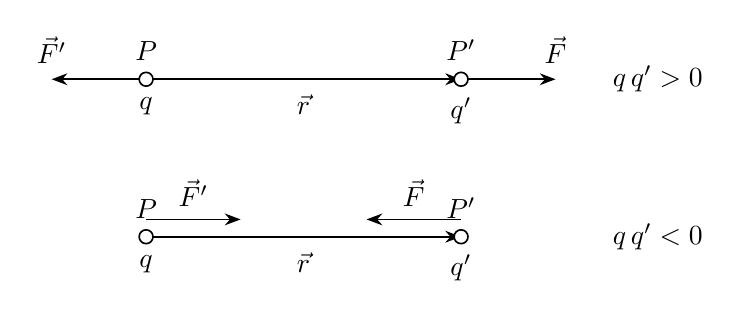
\begin{tikzpicture}[>=Stealth, line width=0.6pt]
    % Caso repulsivo (qq' > 0)
    \begin{scope}[shift={(0,0)}]
      \draw[->] (0,0) -- (4,0) node[midway, below=2pt] {$\vec{r}$};
      
      \draw[->] (0,0) -- (-1.2,0) node[above=2pt] {$\vec{F}'$};
      \draw[->] (4,0) -- (5.2,0) node[above=2pt] {$\vec{F}$};
      
      \filldraw[fill=white, draw=black] (0,0) circle (2.5pt);
      \filldraw[fill=white, draw=black] (4,0) circle (2.5pt);
      
      \node[above=3pt] at (0,0) {$P$};
      \node[below=3pt] at (0,0) {$q$};
      \node[above=3pt] at (4,0) {$P'$};
      \node[below=3pt] at (4,0) {$q'$};
      
      \node[anchor=west] at (5.8,0) {$q\,q' > 0$};
    \end{scope}

    % Caso attrattivo (qq' < 0)
    \begin{scope}[shift={(0,-2.0)}]
      \draw[->] (0,0) -- (4,0) node[midway, below=2pt] {$\vec{r}$};
      
      \draw[->] (0,0.22) -- (1.2,0.22) node[midway, above=1pt] {$\vec{F}'$};
      \draw[->] (4,0.22) -- (2.8,0.22) node[midway, above=1pt] {$\vec{F}$};
      
      \filldraw[fill=white, draw=black] (0,0) circle (2.5pt);
      \filldraw[fill=white, draw=black] (4,0) circle (2.5pt);
      
      \node[above=3pt] at (0,0) {$P$};
      \node[below=3pt] at (0,0) {$q$};
      \node[above=3pt] at (4,0) {$P'$};
      \node[below=3pt] at (4,0) {$q'$};
      
      \node[anchor=west] at (5.8,0) {$q\,q' < 0$};
    \end{scope}
  \end{tikzpicture}
\end{figure}

\end{document}

```

```